\section{Future Work}
\label{sec:future}

While Samba-lite enables experimentation with the proxy re-encryption protocol,
several key tasks remain: \emph{(1)} integrating the runtime into a mainstream
FaaS platform, \emph{(2)} enforcing control-flow integrity at the network I/O
level, and \emph{(3)} extending the function runtime to support trusted
execution environments.
%
We now outline our initial designs for each of these concerns, leaving a
full-fledged design and implementation for future work.


\subsection{Integration with Knative}

\begin{figure}
    \centering
    \includegraphics[page = 6, width=0.48\textwidth]{diagrams/slides.pdf}
    %
    \caption{Knative architecture.
    %
    The Knative components are in light blue.
    %
    The solid arrows are the request flow, and the dashed arrows the
    autoscaling flow.}
    %
    \label{fig:knative}
\end{figure}

\parhead{Knative architecture.}
%
% https://knative.dev/docs/getting-started/next-steps/
% https://knative.dev/docs/serving/architecture/
% https://knative.dev/docs/serving/
%
Knative is a platform-agnostic framework that brings serverless capabilities to
Kubernetes.
%
As Figure~\ref{fig:knative} illustrates, the Knative control plane
consists of an HTTP ingress router, an activator, and an autoscaler.


Under normal traffic,the ingress router routes requests to the activator, which
buffers incoming requests and notifies the autoscaler if additional capacity is
needed; the autoscaler, in turn, requests more pods from Kubernetes.
%
Once new pods are ready---or existing ones become available---the activator
forwards the buffered requests.
%
Under high traffic, the ingress router bypasses the activator and routes
requests directly to the active function pods.
%
Regardless of the traffic pattern, all requests pass through the queue-proxy, a
sidecar container in each function pod.
%
The queue-proxy collects metrics, enforces concurrency limits, and can also
buffer requests when needed, similar to the activator.


To support function chaining, Knative provides an event mesh---an abstraction
of a publish-subscribe system---that enables asynchronous, store-and-forward
message delivery, decoupling senders and recipients in time.


\parhead{\SystemName Knative support.}
%
As the queue-proxy sidecar interposes on the function's I/O, we plan to augment
the sidecar with the functionality for proxy re-encryption and control-flow
enforcement.
%
In this way, the function container itself remains unchanged.




\subsection{Control Flow Integrity}
%
Beyond encrypting function I/O, \SystemName must ensure the integrity
of the sequence of functions.
%
\SystemName approaches this challenge in two ways.
%
First, we will extend the queue-proxy to include a cryptographically binding record
of provenance: each function extends a path signature by signing over its
current link.
%
The last function then posts this provenance record to an untrusted log that
any organization can monitor and audit.
%
Additionally, if an organization knows a flow graph for the function chain (or
some subset thereof),  the queue-proxy will locally verify that the received
event and the function's subsequent output conform to the graph.


\SystemName relies on certificate chains both for attestation and provenance.
%
To reduce bandwidth and storage costs, we will investigate compressing the chains
with an aggregate signature
scheme~\cite{03-eurocrypt-aggregate_signatures_bilinear_maps}.
%
In an \emph{aggregate signature}, each private key $sk_i$ signs a
\emph{distinct} message $m_i$ to form signature $\sigma_i$, and any party can
compress the $\sigma_i$ into a single, small aggregate signature $\sigma^*$.  
%
The aggregate signature convinces a verifier that each signer signed their
respective message.



\subsection{Running Functions in TEEs}

In \SystemName-lite, the function instances run on conventional hardware, thus
allowing the cloud provider to access each function's data, including its keys.
%
To properly address our threat model (which allows for a malicious cloud
provider and cloud-side adversaries), functions must run in secure hardware
enclaves.
%
For future work, we plan to extend \emph{Project Oak},\footnote{
\url{https://github.com/project-oak/oak}
%\url{https://nordprojects.co/projects/oak/}
}
an open-source framework for processing private data within a TEE\@.
%
The central component of Project Oak is the \emph{Oak Functions} platform (see
Figure~\ref{fig:oak}), which executes each function in a confidential VM with a
custom, minimal operating system kernel designed to execute only a single
process.
%
\begin{figure}
    \centering
    \includegraphics[page = 3, width=0.48\textwidth]{diagrams/slides.pdf}
    %
    \caption{Oak and DICE architecture.
    %
    In the DICE model, each software layer loads and measures the next layer,
    generates an ephemeral key pair for the layer, and issues the layer a
    certificate endorsing its measurement and public key.
    %
    Oak uses AMD's trusted hardware as the root of trust.
    %
    % In total, Oak's implementation of DICE results in a certificate chain, rooted
    %in the AMD trusted hardware, that attests the entire workload.
    }
    \label{fig:oak}
\end{figure}
%
The function runs in a secure WebAssembly (Wasm) runtime sandbox, preventing
the process from leaking any sensitive client data.
%
Additionally, Oak uses the DICE~\cite{24-misc-dice} architecture for measured
boot to extend AMD SEV-SNP's attestation from the initial state of the VM
to the entire VM workload.
%

We will modify the Oak kernel to expose critical TEE services---namely,
attestation and sealing---as system calls for the queue-proxy.
%
In this way, the queue-proxy can register its public key with the untrusted
proxy, along with a attestation that binds that key to the function instance.
%
Additionally, sealing enables a leader replica to non-interactively migrate its
key pair to a new leader replica, as during autoscaling operations.




